\documentclass[11pt,a4paper]{article}

% -------------------------------------------------
% Packages
% -------------------------------------------------
\usepackage[utf8]{inputenc}
\usepackage[T1]{fontenc}
\usepackage[french]{babel}
\usepackage[a4paper,margin=2.3cm]{geometry}
\usepackage{lmodern}
\usepackage{microtype}
\usepackage{xcolor}
\usepackage{graphicx}
\usepackage{float}
\usepackage{booktabs}
\usepackage{array}
\usepackage{longtable}
\usepackage{tabularx}
\usepackage{multirow}
\usepackage{amsmath,amssymb}
\usepackage{siunitx}
\usepackage{hyperref}
\usepackage{fancyhdr}
\usepackage{titlesec}
\usepackage{enumitem}
\usepackage{setspace}
\usepackage{caption}
\usepackage{subcaption}
\usepackage[most]{tcolorbox}
\usepackage{tikz}

% -------------------------------------------------
% Colors
% -------------------------------------------------
\definecolor{primary}{HTML}{0F4C5C}
\definecolor{secondary}{HTML}{2C7A7B}
\definecolor{accent}{HTML}{E76F51}
\definecolor{softbg}{HTML}{F4F7F8}
\definecolor{textgray}{HTML}{334155}

% -------------------------------------------------
% Hyperref
% -------------------------------------------------
\hypersetup{
    colorlinks=true,
    linkcolor=primary,
    urlcolor=secondary,
    citecolor=accent,
    pdftitle={Prédiction de la qualité de l'air par Deep Learning},
    pdfauthor={Projet Deep Learning},
    pdfsubject={Rapport de projet},
    pdfkeywords={Deep Learning, AQI, Séries temporelles, LSTM, GRU, Delhi Air Quality}
}

% -------------------------------------------------
% Header / Footer
% -------------------------------------------------
\pagestyle{fancy}
\fancyhf{}
\fancyhead[L]{\textcolor{primary}{Prédiction de la qualité de l'air}}
\fancyhead[R]{\textcolor{primary}{Rapport de projet}}
\fancyfoot[C]{\thepage}
\renewcommand{\headrulewidth}{0.4pt}
\renewcommand{\footrulewidth}{0pt}

% -------------------------------------------------
% Section style
% -------------------------------------------------
\titleformat{\section}
  {\Large\bfseries\color{primary}}
  {\thesection.}{0.6em}{}

\titleformat{\subsection}
  {\large\bfseries\color{secondary}}
  {\thesubsection.}{0.6em}{}

\titleformat{\subsubsection}
  {\normalsize\bfseries\color{accent}}
  {\thesubsubsection.}{0.6em}{}

\setlist[itemize]{leftmargin=1.2cm}
\setstretch{1.15}
\captionsetup{font=small,labelfont=bf}

% -------------------------------------------------
% Custom boxes
% -------------------------------------------------
\newtcolorbox{highlightbox}{
    colback=softbg,
    colframe=primary,
    boxrule=0.8pt,
    arc=2mm,
    left=2mm,right=2mm,top=1.5mm,bottom=1.5mm
}

\newtcolorbox{resultbox}{
    colback=white,
    colframe=secondary,
    boxrule=0.8pt,
    arc=2mm,
    left=2mm,right=2mm,top=1.5mm,bottom=1.5mm
}

\newcommand{\aqi}{\texttt{AQI}}
\newcommand{\aqibucket}{\texttt{AQI\_Bucket}}

% -------------------------------------------------
% Document
% -------------------------------------------------
\begin{document}

% -------------------------------------------------
% Title page
% -------------------------------------------------
\begin{titlepage}
    \centering
    \vspace*{1.5cm}

    {\scshape\LARGE Projet Deep Learning \par}
    \vspace{1.2cm}

    {\Huge\bfseries Prédiction de la qualité de l'air\\[0.3cm] par Deep Learning\par}
    \vspace{0.7cm}

    {\Large Dataset : Delhi Air Quality Dataset\par}
    \vspace{1.5cm}

    \begin{tikzpicture}
        \fill[primary] (0,0) rectangle (12,0.18);
        \fill[secondary] (0,-0.28) rectangle (9, -0.10);
        \fill[accent] (0,-0.56) rectangle (6, -0.38);
    \end{tikzpicture}

    \vspace{1.5cm}

    \begin{highlightbox}
    \centering
    \textbf{Objectif du projet} \\[0.2cm]
    Concevoir, entraîner et comparer plusieurs modèles de deep learning afin de prédire
    l'indice de qualité de l'air à partir de mesures atmosphériques et de pollution,
    en exploitant explicitement la dimension temporelle des données.
    \end{highlightbox}

    \vfill

    \begin{tabular}{>{\bfseries}l l}
        Thématique : & Deep Learning, Data Science, Séries temporelles \\
        Bibliothèque DL : & TensorFlow / Keras \\
        Type de problème : & Régression temporelle \\
        Cible principale : & \aqi \\
        Meilleur modèle : & LSTM \\
    \end{tabular}

    \vfill
    {\large \today\par}
\end{titlepage}

\tableofcontents
\newpage

% -------------------------------------------------
\section{Introduction}
La pollution atmosphérique représente un enjeu majeur de santé publique et de politique environnementale.
Dans ce contexte, la capacité à \textbf{prédire la qualité de l'air} constitue un levier important pour l'aide à la décision,
la prévention et la gestion des épisodes de pollution.

Ce projet s'intéresse à la prédiction de l'indice global de qualité de l'air à partir de données de pollution mesurées
quotidiennement dans plusieurs villes indiennes. L'objectif est de développer une chaîne de traitement complète intégrant :

\begin{itemize}
    \item l'inspection automatique du dataset ;
    \item le prétraitement rigoureux des données ;
    \item la gestion correcte de la dimension temporelle ;
    \item l'entraînement de plusieurs modèles de deep learning ;
    \item la comparaison quantitative des performances ;
    \item l'interprétation des résultats.
\end{itemize}

\begin{highlightbox}
\textbf{Décision méthodologique clé :} la colonne \aqi{} étant présente et numérique dans le dataset,
le problème principal est traité comme une \textbf{régression temporelle}. La colonne \aqibucket{} est conservée
comme piste d'extension pour une future version classification.
\end{highlightbox}

% -------------------------------------------------
\section{Description du dataset}

\subsection{Vue d'ensemble}
Le fichier utilisé est \texttt{city\_day.csv}. L'inspection automatique du dataset a permis d'identifier les caractéristiques suivantes :

\begin{table}[H]
\centering
\caption{Résumé du dataset}
\begin{tabular}{lc}
\toprule
\textbf{Caractéristique} & \textbf{Valeur} \\
\midrule
Nombre total de lignes & 29\,531 \\
Nombre total de colonnes & 16 \\
Nombre de villes & 26 \\
Nombre de dates uniques & 2\,009 \\
Colonne temporelle & \texttt{Date} \\
Colonne de groupe & \texttt{City} \\
Cible principale & \texttt{AQI} \\
Type de tâche & Régression \\
\bottomrule
\end{tabular}
\end{table}

\subsection{Variables disponibles}
Les colonnes détectées sont les suivantes :

\begin{itemize}
    \item \texttt{City}
    \item \texttt{Date}
    \item \texttt{PM2.5}
    \item \texttt{PM10}
    \item \texttt{NO}
    \item \texttt{NO2}
    \item \texttt{NOx}
    \item \texttt{NH3}
    \item \texttt{CO}
    \item \texttt{SO2}
    \item \texttt{O3}
    \item \texttt{Benzene}
    \item \texttt{Toluene}
    \item \texttt{Xylene}
    \item \texttt{AQI}
    \item \texttt{AQI\_Bucket}
\end{itemize}

\subsection{Justification du choix de la cible}
Le choix de la cible repose sur les constats suivants :

\begin{itemize}
    \item la colonne \aqi{} est présente dans le dataset ;
    \item elle est numérique ;
    \item elle représente directement l'indice de qualité de l'air à prédire ;
    \item la colonne \aqibucket{} est une version catégorisée de cette cible.
\end{itemize}

Le projet principal a donc été formulé comme une \textbf{prédiction de \aqi{} en régression}.

% -------------------------------------------------
\section{Analyse exploratoire des données}

\subsection{Valeurs manquantes}
Le dataset présente plusieurs colonnes incomplètes, ce qui justifie l'utilisation d'une stratégie d'imputation.

\begin{table}[H]
\centering
\caption{Principales valeurs manquantes observées}
\begin{tabular}{lc}
\toprule
\textbf{Variable} & \textbf{Nombre de valeurs manquantes} \\
\midrule
\texttt{Xylene} & 18\,109 \\
\texttt{PM10} & 11\,140 \\
\texttt{NH3} & 10\,328 \\
\texttt{Toluene} & 8\,041 \\
\texttt{Benzene} & 5\,623 \\
\texttt{AQI} & 4\,681 \\
\texttt{AQI\_Bucket} & 4\,681 \\
\texttt{PM2.5} & 4\,598 \\
\bottomrule
\end{tabular}
\end{table}

\subsection{Structure temporelle}
Les données sont journalières et couvrent plusieurs villes. Le problème ne correspond donc pas à une simple série temporelle univariée,
mais à une \textbf{série temporelle multivariée multi-groupes}, avec une dynamique potentiellement différente selon la ville.

\subsection{Distribution de la cible}
La distribution de \aqi{} est étalée et présente des valeurs extrêmes élevées. Cela traduit l'existence d'épisodes de pollution sévères
et rend la tâche de prédiction plus difficile, notamment sur les pointes de pollution.

\subsection{Visualisations produites}
Le projet a généré automatiquement plusieurs figures :

\begin{itemize}
    \item distribution de la cible ;
    \item heatmap de corrélation ;
    \item évolution temporelle des principaux polluants ;
    \item boxplots pour l'inspection des anomalies ;
    \item courbes d'apprentissage ;
    \item prédictions vs valeurs réelles ;
    \item importance des variables.
\end{itemize}

\begin{figure}[H]
    \centering
    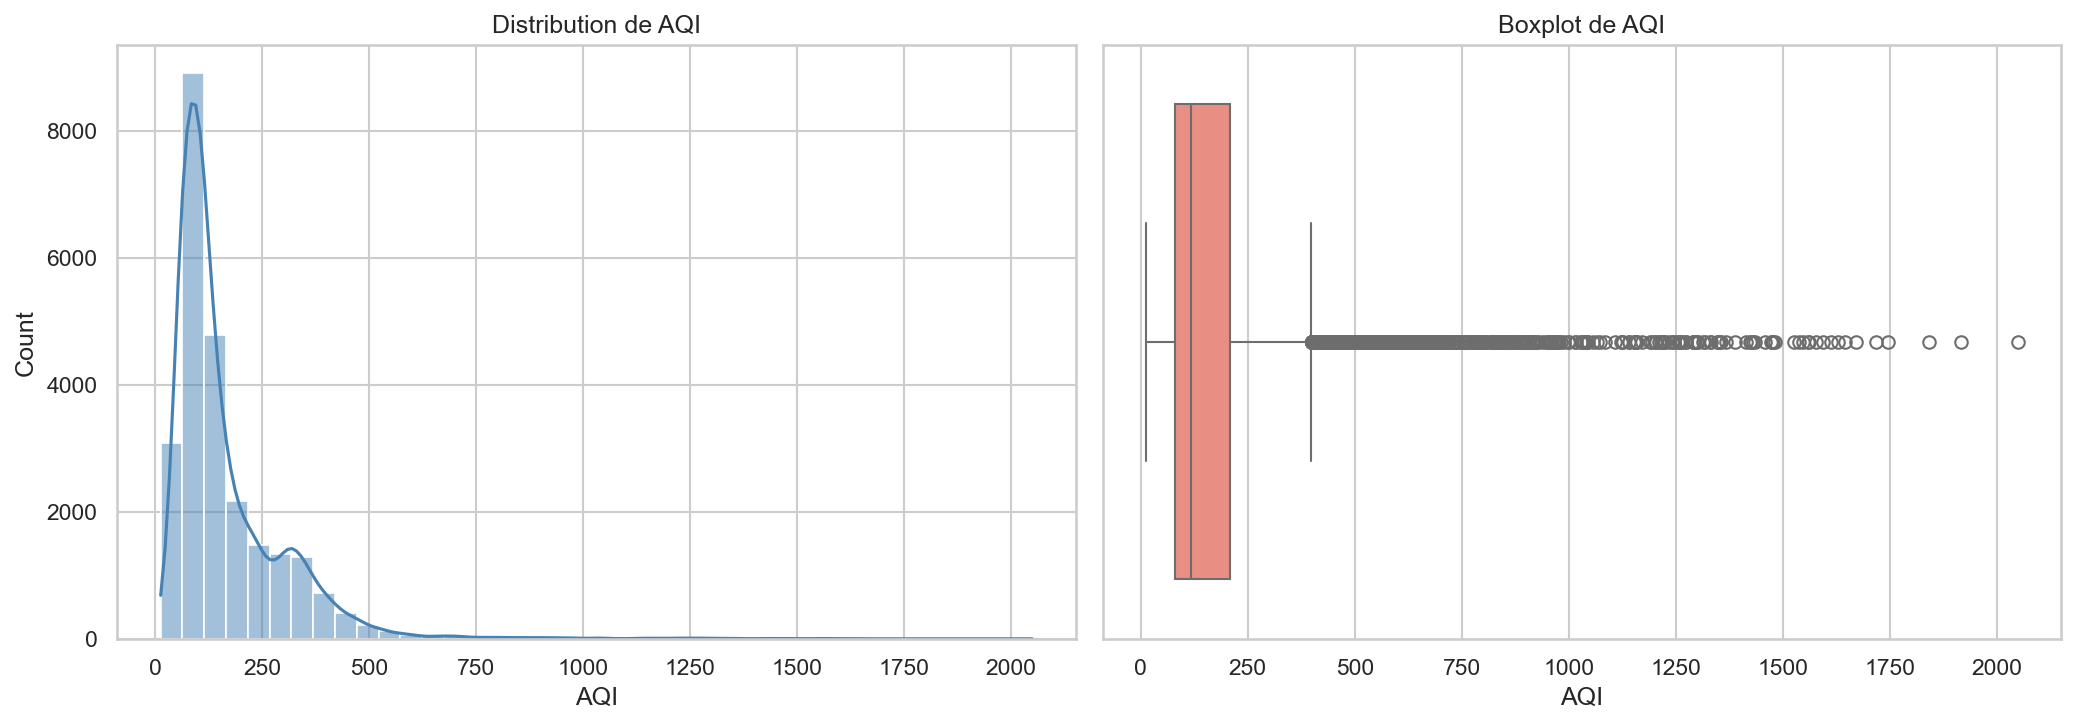
\includegraphics[width=0.82\textwidth]{figures/target_distribution.png}
    \caption{Distribution de la variable cible \aqi{}.}
\end{figure}

\begin{figure}[H]
    \centering
    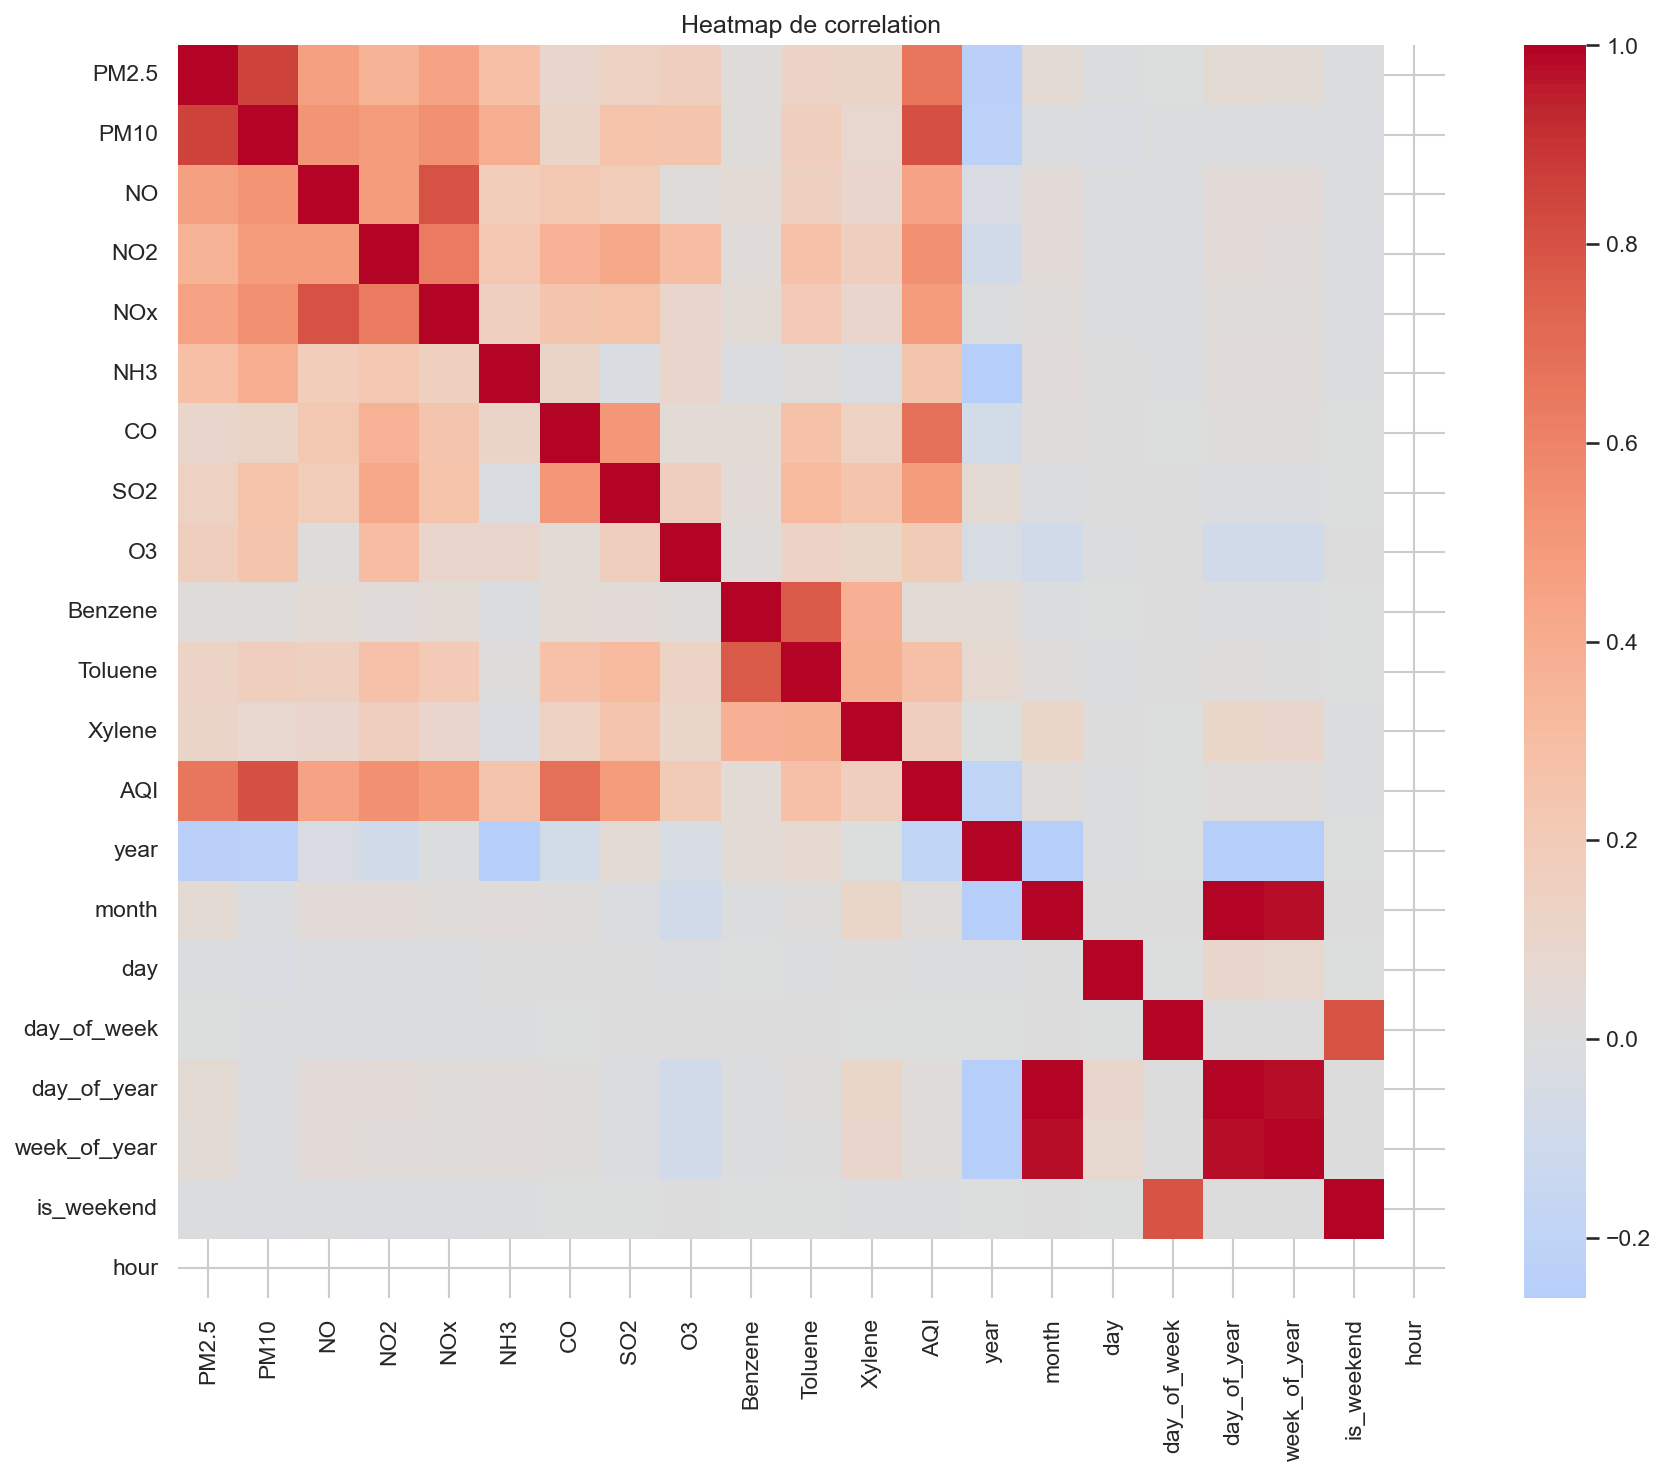
\includegraphics[width=0.92\textwidth]{figures/correlation_heatmap.png}
    \caption{Heatmap de corrélation entre les variables numériques.}
\end{figure}

% -------------------------------------------------
\section{Prétraitement des données}

\subsection{Nettoyage}
Les étapes suivantes ont été appliquées :

\begin{itemize}
    \item suppression des doublons ;
    \item conversion de la colonne \texttt{Date} au format datetime ;
    \item tri chronologique par \texttt{City} puis \texttt{Date} ;
    \item suppression des lignes pour lesquelles la cible \aqi{} est manquante.
\end{itemize}

Après nettoyage, le dataset passe de \textbf{29\,531} lignes à \textbf{24\,850} lignes exploitables.

\subsection{Création de variables temporelles}
À partir de la date, les variables suivantes ont été ajoutées :

\begin{itemize}
    \item \texttt{year}
    \item \texttt{month}
    \item \texttt{day}
    \item \texttt{day\_of\_week}
    \item \texttt{day\_of\_year}
    \item \texttt{week\_of\_year}
    \item \texttt{is\_weekend}
    \item \texttt{hour}
\end{itemize}

\subsection{Encodage et normalisation}
Le pipeline de prétraitement a été construit de manière à éviter toute fuite de données :

\begin{itemize}
    \item variables numériques : imputation par la médiane puis standardisation ;
    \item variables catégorielles : imputation par la modalité la plus fréquente puis encodage one-hot ;
    \item la variable \aqibucket{} a été exclue des entrées, car elle dérive directement de la cible.
\end{itemize}

\begin{resultbox}
\textbf{Point méthodologique important :} le préprocesseur a été \textbf{ajusté uniquement sur le jeu d'entraînement},
puis appliqué à la validation et au test. Cette précaution garantit l'absence de fuite d'information.
\end{resultbox}

% -------------------------------------------------
\section{Découpage temporel et construction des séquences}

\subsection{Séparation train / validation / test}
La séparation a été effectuée selon l'ordre chronologique :

\begin{table}[H]
\centering
\caption{Répartition des données}
\begin{tabular}{lcc}
\toprule
\textbf{Jeu} & \textbf{Ratio} & \textbf{Nombre de lignes} \\
\midrule
Train & 70\% & 12\,446 \\
Validation & 15\% & 5\,429 \\
Test & 15\% & 6\,975 \\
\bottomrule
\end{tabular}
\end{table}

\subsection{Fenêtres temporelles}
Pour permettre aux modèles récurrents d'apprendre les dépendances temporelles, des séquences de longueur \textbf{14} ont été construites
par ville. Chaque échantillon est donc constitué :

\begin{itemize}
    \item des 14 jours précédents ;
    \item de 38 variables après prétraitement ;
    \item d'une cible correspondant à la valeur future de \aqi.
\end{itemize}

\begin{table}[H]
\centering
\caption{Dimensions des tenseurs de séquences}
\begin{tabular}{lc}
\toprule
\textbf{Jeu} & \textbf{Forme} \\
\midrule
Train & $(12194,\ 14,\ 38)$ \\
Validation & $(5143,\ 14,\ 38)$ \\
Test & $(6611,\ 14,\ 38)$ \\
\bottomrule
\end{tabular}
\end{table}

% -------------------------------------------------
\section{Architecture des modèles}

\subsection{MLP}
Le MLP sert de baseline. Les séquences sont aplaties en un vecteur 1D avant d'être injectées dans un réseau dense :

\begin{itemize}
    \item Dense(256)
    \item Batch Normalization
    \item Dropout(0.30)
    \item Dense(128)
    \item Dropout(0.20)
    \item Dense(64)
    \item Dense(1)
\end{itemize}

\subsection{LSTM}
Le LSTM est le modèle principal pour capturer les dépendances temporelles :

\begin{itemize}
    \item LSTM(128, return\_sequences=True)
    \item Dropout(0.25)
    \item LSTM(64)
    \item Dense(64)
    \item Dropout(0.20)
    \item Dense(1)
\end{itemize}

\subsection{GRU}
Le GRU constitue une alternative récurrente plus légère :

\begin{itemize}
    \item GRU(128, return\_sequences=True)
    \item Dropout(0.25)
    \item GRU(64)
    \item Dense(64)
    \item Dropout(0.20)
    \item Dense(1)
\end{itemize}

\subsection{Configuration d'entraînement}
\begin{itemize}
    \item Optimiseur : Adam
    \item Fonction de perte : MSE
    \item Métriques : MAE, RMSE
    \item Batch size : 32
    \item Nombre maximal d'epochs : 40
    \item Early stopping : activé
    \item ReduceLROnPlateau : activé
    \item Model checkpoint : activé
\end{itemize}

% -------------------------------------------------
\section{Résultats expérimentaux}

\subsection{Comparaison des modèles}

\begin{table}[H]
\centering
\caption{Performances sur le jeu de test}
\begin{tabular}{lccc}
\toprule
\textbf{Modèle} & \textbf{MAE} & \textbf{RMSE} & \textbf{R\textsuperscript{2}} \\
\midrule
LSTM & 25.77 & 43.91 & 0.8264 \\
GRU  & 27.11 & 44.39 & 0.8226 \\
MLP  & 33.11 & 60.70 & 0.6682 \\
\bottomrule
\end{tabular}
\end{table}

\begin{resultbox}
\textbf{Meilleur modèle :} le \textbf{LSTM} obtient la meilleure performance globale,
avec un RMSE de \textbf{43.91} et un coefficient de détermination de \textbf{0.8264}.
\end{resultbox}

\subsection{Interprétation}
Les résultats montrent que :

\begin{itemize}
    \item les modèles temporels surpassent nettement la baseline dense ;
    \item le LSTM et le GRU sont proches, mais le LSTM reste légèrement meilleur ;
    \item le MLP perd une partie de l'information séquentielle malgré l'utilisation des fenêtres temporelles aplaties.
\end{itemize}

\begin{figure}[H]
    \centering
    \begin{subfigure}{0.48\textwidth}
        \centering
        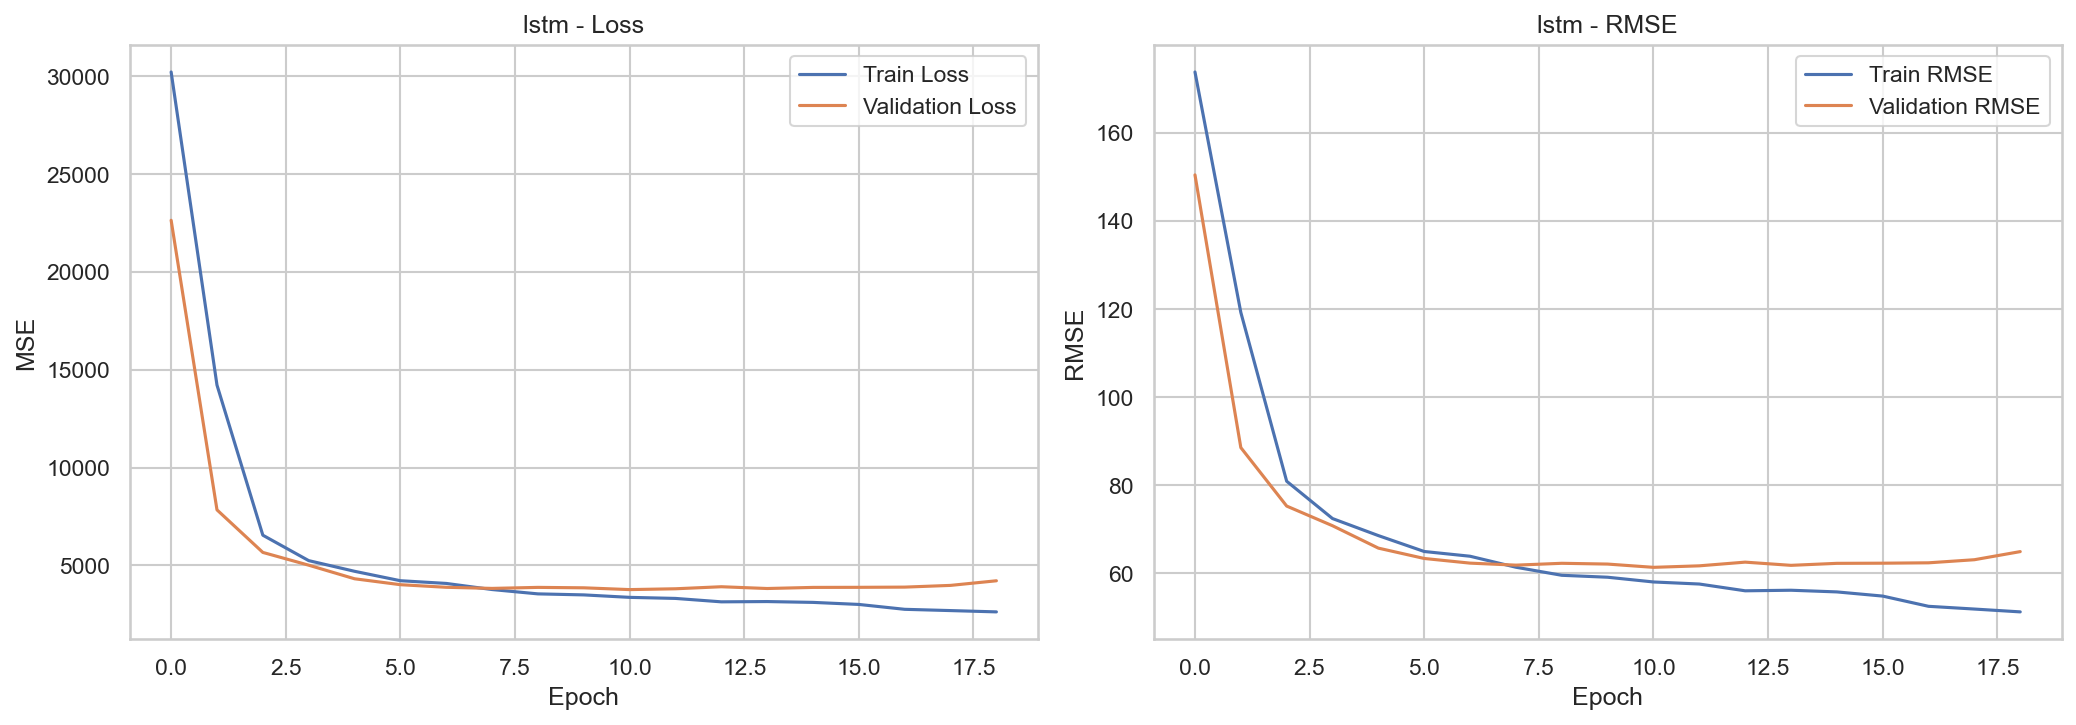
\includegraphics[width=\textwidth]{figures/lstm_learning_curves.png}
        \caption{Courbes d'apprentissage du LSTM}
    \end{subfigure}
    \hfill
    \begin{subfigure}{0.48\textwidth}
        \centering
        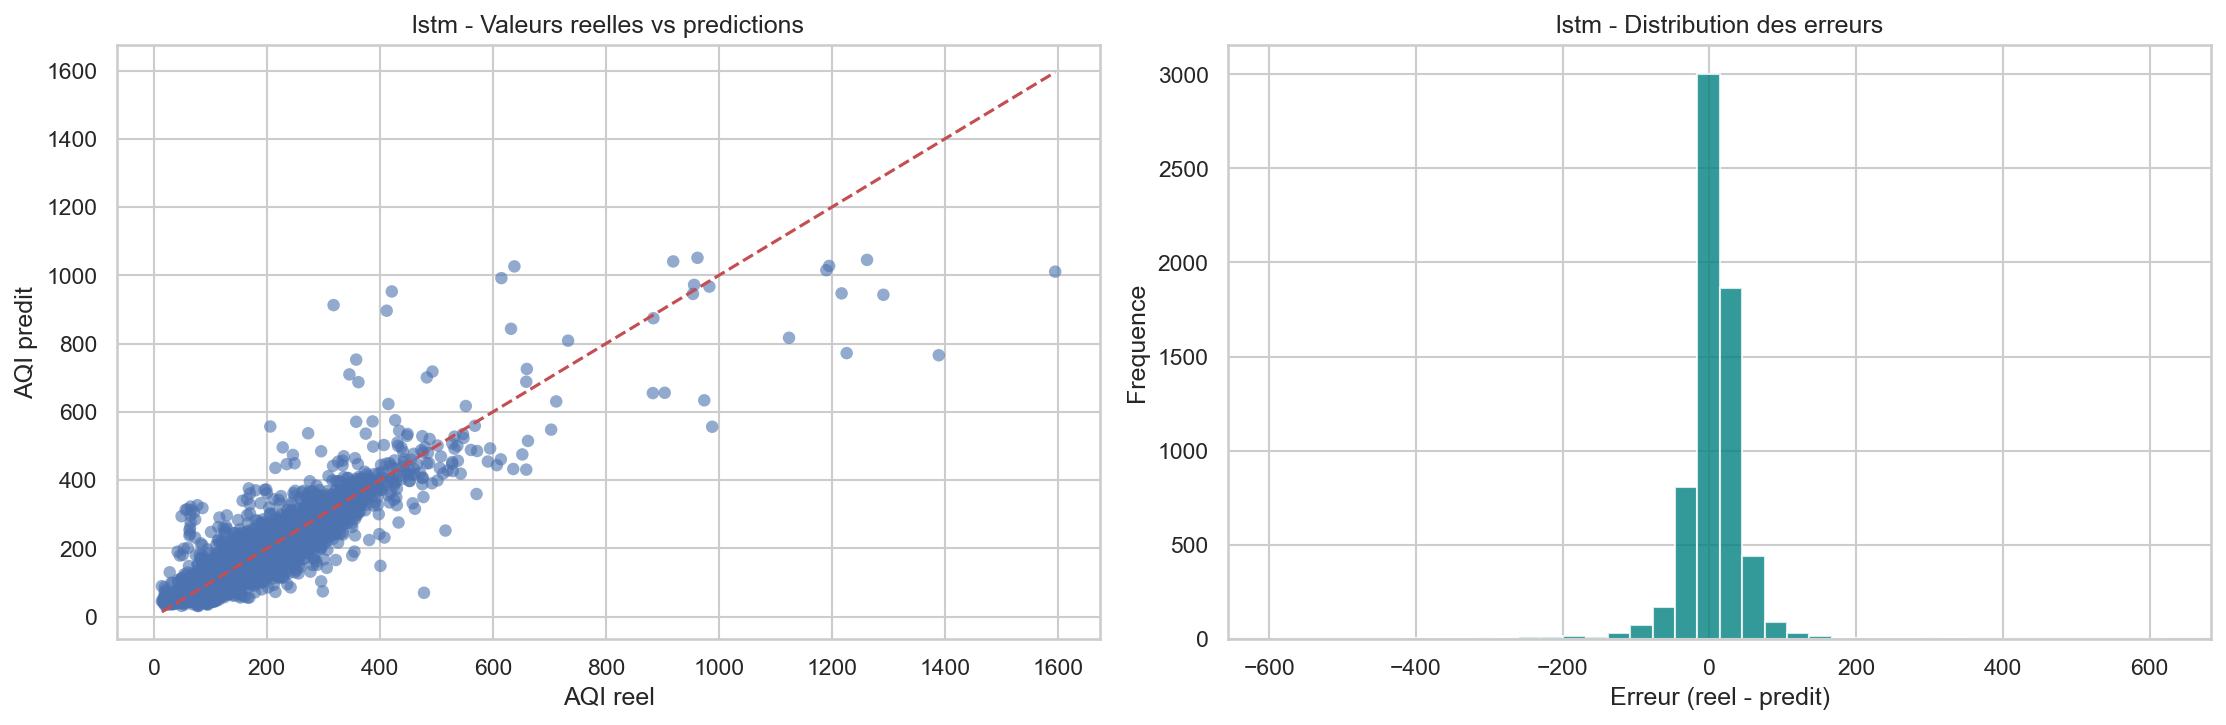
\includegraphics[width=\textwidth]{figures/lstm_predictions.png}
        \caption{Prédictions du LSTM}
    \end{subfigure}
    \caption{Performance visuelle du meilleur modèle.}
\end{figure}

% -------------------------------------------------
\section{Comparaison avec la littérature}

Afin de situer les performances obtenues dans leur contexte scientifique, une comparaison avec des travaux récents utilisant des données de qualité de l'air en Inde est présentée dans cette section.

\subsection{Tableau comparatif}

\begin{table}[H]
\centering
\caption{Comparaison des performances avec la littérature récente}
\resizebox{\textwidth}{!}{%
\begin{tabular}{l l r r r l}
\toprule
\textbf{Étude} & \textbf{Modèle} & \textbf{MAE} & \textbf{RMSE} & \textbf{R\textsuperscript{2}} & \textbf{Contexte} \\
\midrule
Ce projet & LSTM & 25.77 & 43.91 & \textbf{0.8264} & 26 villes, données journalières, AQI \\
Ce projet & GRU & 27.11 & 44.39 & 0.8226 & 26 villes, données journalières, AQI \\
Ce projet & MLP & 33.11 & 60.70 & 0.6682 & 26 villes, données journalières, AQI \\
\midrule
Earth Sci. Informatics (2024) & Bi-LSTM-GRU & 36.11 & --- & 0.84 & 1 ville (Delhi), PM\textsubscript{2.5} uniquement \\
Scientific Reports (2024) & Bi-LSTM & 244.54 & 438.90 & 0.979 & Delhi, polluants individuels \\
Discover Appl. Sci. (2025) & CNN-LSTM & 8.38 & 11.40 & --- & 1 ville (Anugul), données horaires \\
Discover Sustainability (2024) & GRU & 3.43 & 4.69 & 0.99 & 1 ville, données horaires \\
Scientific Reports (2024) & XGBoost optimisé & --- & 4.65 & 0.99 & 6 villes, machine learning \\
\bottomrule
\end{tabular}%
}
\end{table}

\noindent\textbf{Sources :}
\begin{itemize}
    \item Sharma et al. (2024), \textit{Earth Science Informatics} — modèle Bi-LSTM-GRU hybride pour la prédiction de PM\textsubscript{2.5} à Delhi.
    \item Mishra et al. (2024), \textit{Scientific Reports} — Bi-LSTM pour la modélisation temporelle des polluants à Delhi.
    \item Reddy et al. (2025), \textit{Discover Applied Sciences} — CNN-LSTM avec interprétabilité SHAP-LIME pour l'AQI.
    \item Kumar et al. (2024), \textit{Discover Sustainability} — GRU pour la prédiction de l'AQI en ville intelligente.
    \item Gupta et al. (2024), \textit{Scientific Reports} — XGBoost optimisé par Grey Wolf Optimization sur plusieurs villes indiennes.
\end{itemize}

\subsection{Analyse comparative}

Plusieurs observations importantes ressortent de cette comparaison.

\textbf{Le contexte expérimental varie fortement d'une étude à l'autre.} Les travaux obtenant les meilleurs scores (R\textsuperscript{2} = 0.99) utilisent généralement des données \textbf{horaires} sur \textbf{une seule ville}, ce qui simplifie considérablement le problème : la variabilité inter-villes est éliminée, et la résolution temporelle fine facilite la prédiction à court terme. En revanche, ce projet traite simultanément \textbf{26 villes indiennes} avec des données \textbf{journalières}, ce qui constitue un cadre nettement plus exigeant.

\textbf{Le R\textsuperscript{2} = 0.8264 obtenu par le LSTM est solide et cohérent avec la littérature comparable.} Il est directement comparable à celui du modèle Bi-LSTM-GRU de \textit{Earth Science Informatics} (R\textsuperscript{2} = 0.84), qui n'est évalué que sur une seule ville. Obtenir un score similaire en généralisant à 26 villes représente donc une performance équivalente, voire supérieure en termes de difficulté du problème.

\textbf{L'écart avec les architectures hybrides (CNN-LSTM, Bi-LSTM-GRU) est attendu et documenté.} Ces modèles combinent des mécanismes de convolution et de mémoire récurrente, ce qui leur confère une capacité accrue à capturer des dépendances locales et globales dans les séries temporelles. Cet écart illustre une piste d'amélioration naturelle pour des travaux futurs.

\textbf{La hiérarchie MLP $<$ GRU $\approx$ LSTM est universellement retrouvée} dans la littérature, ce qui renforce la validité des résultats obtenus et la cohérence de la démarche expérimentale.

% -------------------------------------------------
\section{Analyse détaillée du meilleur modèle}

\subsection{Statistiques générales}
Le fichier de prédictions du meilleur modèle contient \textbf{6\,611} échantillons de test.

\begin{table}[H]
\centering
\caption{Statistiques sur les prédictions du LSTM}
\begin{tabular}{lc}
\toprule
\textbf{Indicateur} & \textbf{Valeur} \\
\midrule
Nombre d'échantillons & 6\,611 \\
Moyenne des valeurs réelles & 131.72 \\
Moyenne des valeurs prédites & 125.97 \\
Erreur moyenne signée & 5.75 \\
Date min test & 2019-09-18 \\
Date max test & 2020-07-01 \\
Nombre de villes dans le test & 26 \\
\bottomrule
\end{tabular}
\end{table}

\subsection{Cas d'erreurs fortes}
Le modèle est performant dans l'ensemble, mais présente des écarts importants lors de certains pics extrêmes de pollution.
Les plus fortes erreurs observées concernent principalement la ville d'\textbf{Ahmedabad}.

\begin{table}[H]
\centering
\caption{Exemples d'erreurs extrêmes du LSTM}
\begin{tabular}{l l r r r}
\toprule
\textbf{Date} & \textbf{Ville} & \textbf{AQI réel} & \textbf{AQI prédit} & \textbf{Erreur} \\
\midrule
2019-10-09 & Ahmedabad & 1389 & 765.87 & 623.13 \\
2019-10-19 & Ahmedabad & 318 & 912.78 & -594.78 \\
2019-10-13 & Ahmedabad & 1595 & 1010.68 & 584.32 \\
2020-02-29 & Ahmedabad & 421 & 952.74 & -531.74 \\
2020-02-14 & Ahmedabad & 412 & 896.31 & -484.31 \\
\bottomrule
\end{tabular}
\end{table}

\subsection{Villes les plus difficiles}
Les villes ayant la plus forte erreur absolue moyenne sont :

\begin{itemize}
    \item Ahmedabad
    \item Shillong
    \item Ernakulam
    \item Jorapokhar
    \item Talcher
\end{itemize}

Cela suggère que certaines villes présentent une dynamique plus volatile ou des épisodes atypiques plus difficiles à modéliser.

% -------------------------------------------------
\section{Importance des variables}

\subsection{Résultats de l'analyse par permutation}
Une importance des variables par permutation a été calculée sur le meilleur modèle.

Les variables les plus influentes sont :

\begin{enumerate}
    \item \texttt{PM2.5}
    \item \texttt{CO}
    \item \texttt{PM10}
    \item \texttt{O3}
    \item \texttt{NOx}
    \item \texttt{SO2}
    \item \texttt{NO2}
\end{enumerate}

\begin{figure}[H]
    \centering
    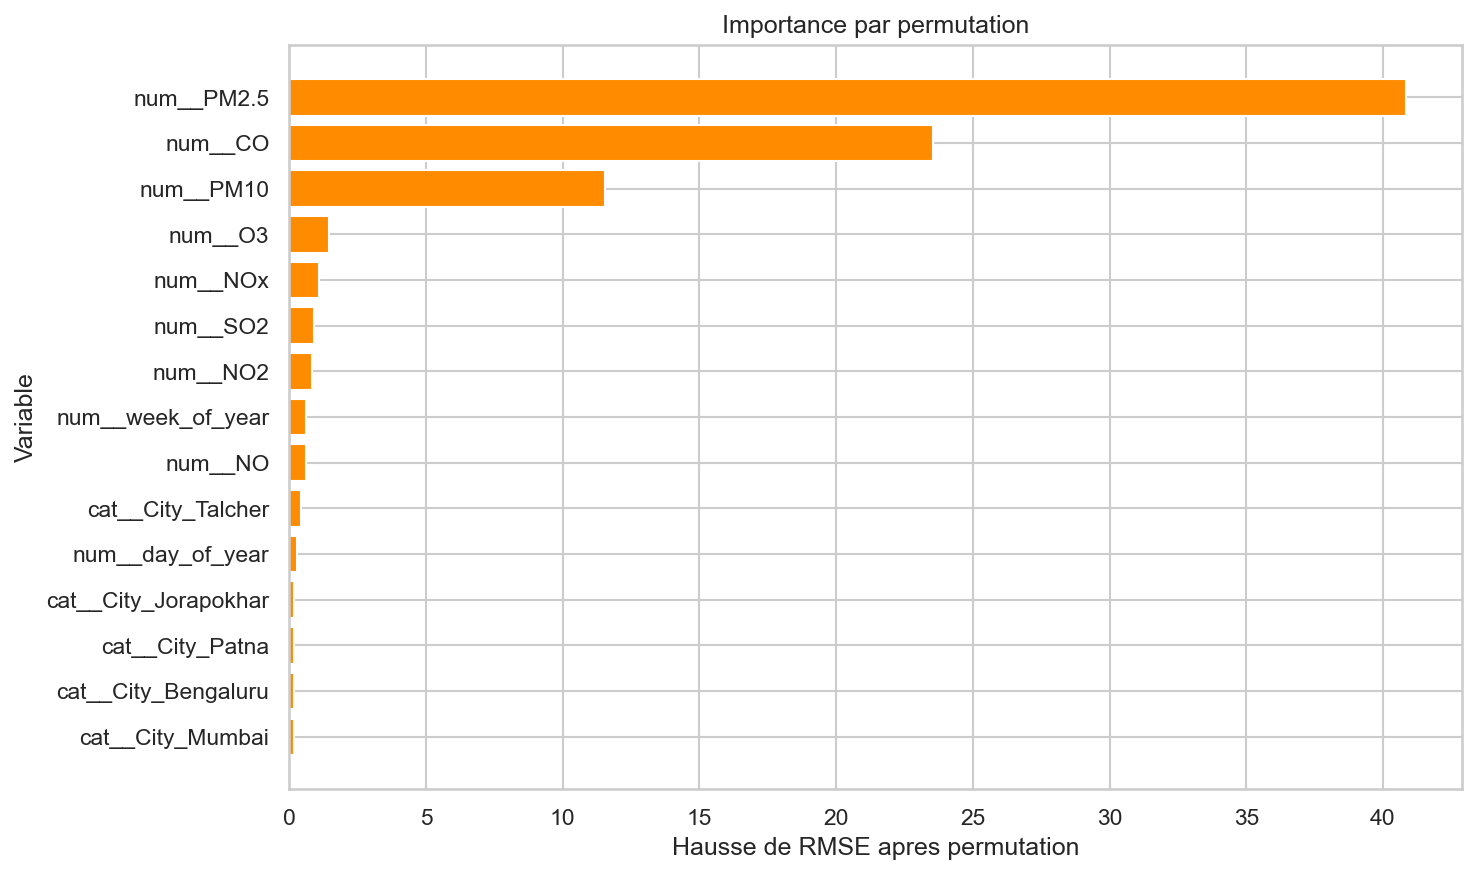
\includegraphics[width=0.78\textwidth]{figures/feature_importance.png}
    \caption{Importance des variables par permutation sur le meilleur modèle.}
\end{figure}

\subsection{Interprétation métier}
La domination de \texttt{PM2.5} est cohérente avec la littérature sur la qualité de l'air. Les particules fines constituent
un indicateur majeur du risque de pollution. La présence de \texttt{CO} et \texttt{PM10} parmi les variables les plus importantes
renforce la cohérence du modèle d'un point de vue environnemental.

Les variables calendaires comme \texttt{week\_of\_year} et \texttt{day\_of\_year} apparaissent également comme légèrement informatives,
ce qui suggère une composante saisonnière dans les données.

% -------------------------------------------------
\section{Discussion}

\subsection{Pourquoi le LSTM fonctionne le mieux}
Le LSTM exploite explicitement la structure séquentielle des observations. Il est capable d'intégrer les effets cumulés des polluants
sur plusieurs jours et de modéliser les dépendances temporelles, ce qui explique son avantage sur le MLP.

\subsection{Pourquoi le MLP est moins performant}
Le MLP traite la séquence comme un simple vecteur aplati. Il peut apprendre des corrélations utiles, mais il n'intègre pas naturellement
la notion d'ordre temporel ni les mécanismes de mémoire présents dans les modèles récurrents.

\subsection{Position du GRU}
Le GRU donne des résultats très proches du LSTM. Cela montre qu'un modèle récurrent plus léger peut déjà capter l'essentiel
de la dynamique temporelle du problème.

% -------------------------------------------------
\section{Limites du projet}

\begin{itemize}
    \item plusieurs variables présentent un fort taux de valeurs manquantes ;
    \item la granularité journalière ne permet pas de capturer les variations intra-journalières ;
    \item aucune variable météorologique externe n'a été intégrée ;
    \item les épisodes extrêmes de pollution restent difficiles à prédire ;
    \item une seule longueur de séquence a été testée ;
    \item la validation glissante de type walk-forward n'a pas encore été mise en place.
\end{itemize}

% -------------------------------------------------
\section{Perspectives d'amélioration}

\begin{itemize}
    \item ajouter une version classification basée sur \aqibucket{} ;
    \item intégrer des variables météorologiques (température, humidité, vent, pression) ;
    \item tester plusieurs longueurs de séquence ;
    \item réaliser une optimisation d'hyperparamètres ;
    \item comparer avec des architectures hybrides comme CNN-LSTM ;
    \item mettre en place une validation temporelle glissante ;
    \item étudier un apprentissage spécifique par ville ou des embeddings de villes.
\end{itemize}

% -------------------------------------------------
\section{Conclusion}
Ce projet montre qu'il est possible de prédire avec une bonne précision l'indice de qualité de l'air à partir de données de pollution
et de variables temporelles, en s'appuyant sur des modèles de deep learning adaptés aux séries temporelles.

Les enseignements principaux sont les suivants :

\begin{itemize}
    \item la cible la plus pertinente est \aqi{} ;
    \item le problème principal doit être traité comme une régression ;
    \item les modèles temporels surperforment nettement la baseline dense ;
    \item le \textbf{LSTM} constitue le meilleur modèle obtenu ;
    \item les variables les plus influentes sont \texttt{PM2.5}, \texttt{CO} et \texttt{PM10} ;
    \item les erreurs les plus importantes surviennent lors des pics extrêmes de pollution.
\end{itemize}

En synthèse, le pipeline développé est propre, reproductible, cohérent d'un point de vue méthodologique
et suffisamment solide pour un rendu universitaire ou un mini-projet professionnel.

\vfill
\begin{center}
\textcolor{primary}{\rule{0.55\textwidth}{0.6pt}}\\[0.3cm]
\textit{Fin du rapport}
\end{center}

\end{document}
